%%%%%%%%%%%%%%%%%%%%%%%%%%%%%%%%%%%%%%%%%
% Beamer Presentation
% LaTeX Template
% Version 2.0 (March 8, 2022)
%
% This template originates from:
% https://www.LaTeXTemplates.com
%
% Author:
% Vel (vel@latextemplates.com)
%
% License:
% CC BY-NC-SA 4.0 (https://creativecommons.org/licenses/by-nc-sa/4.0/)
%
%%%%%%%%%%%%%%%%%%%%%%%%%%%%%%%%%%%%%%%%%

%----------------------------------------------------------------------------------------
%	PACKAGES AND OTHER DOCUMENT CONFIGURATIONS
%----------------------------------------------------------------------------------------

\documentclass[
	11pt, % Set the default font size, options include: 8pt, 9pt, 10pt, 11pt, 12pt, 14pt, 17pt, 20pt
	%t, % Uncomment to vertically align all slide content to the top of the slide, rather than the default centered
	%aspectratio=169, % Uncomment to set the aspect ratio to a 16:9 ratio which matches the aspect ratio of 1080p and 4K screens and projectors
]{beamer}

\graphicspath{{Images/}{./}} % Specifies where to look for included images (trailing slash required)

\usepackage{booktabs} % Allows the use of \toprule, \midrule and \bottomrule for better rules in tables
\usepackage[russian]{babel}
% \usepackage[english,russian]{babel}
\usepackage[dvipsnames]{xcolor}
\usepackage{xcolor}

%----------------------------------------------------------------------------------------
%	SELECT LAYOUT THEME
%----------------------------------------------------------------------------------------

% Beamer comes with a number of default layout themes which change the colors and layouts of slides. Below is a list of all themes available, uncomment each in turn to see what they look like.

%\usetheme{default}
%\usetheme{AnnArbor}
%\usetheme{Antibes}
%\usetheme{Bergen}
%\usetheme{Berkeley}
%\usetheme{Berlin}
%\usetheme{Boadilla}
%\usetheme{CambridgeUS}
%\usetheme{Copenhagen}
%\usetheme{Darmstadt}
%\usetheme{Dresden}
%\usetheme{Frankfurt}
%\usetheme{Goettingen}
%\usetheme{Hannover}
%\usetheme{Ilmenau}
%\usetheme{JuanLesPins}
%\usetheme{Luebeck}
\usetheme{Madrid}
%\usetheme{Malmoe}
%\usetheme{Marburg}
%\usetheme{Montpellier}
%\usetheme{PaloAlto}
%\usetheme{Pittsburgh}
%\usetheme{Rochester}
%\usetheme{Singapore}
%\usetheme{Szeged}
%\usetheme{Warsaw}

%----------------------------------------------------------------------------------------
%	SELECT COLOR THEME
%----------------------------------------------------------------------------------------

% Beamer comes with a number of color themes that can be applied to any layout theme to change its colors. Uncomment each of these in turn to see how they change the colors of your selected layout theme.

%\usecolortheme{albatross}
%\usecolortheme{beaver}
%\usecolortheme{beetle}
%\usecolortheme{crane}
%\usecolortheme{dolphin}
%\usecolortheme{dove}
%\usecolortheme{fly}
%\usecolortheme{lily}
%\usecolortheme{monarca}
%\usecolortheme{seagull}
%\usecolortheme{seahorse}
%\usecolortheme{spruce}
%\usecolortheme{whale}
%\usecolortheme{wolverine}

%----------------------------------------------------------------------------------------
%	SELECT FONT THEME & FONTS
%----------------------------------------------------------------------------------------

% Beamer comes with several font themes to easily change the fonts used in various parts of the presentation. Review the comments beside each one to decide if you would like to use it. Note that additional options can be specified for several of these font themes, consult the beamer documentation for more information.

\usefonttheme{default} % Typeset using the default sans serif font
%\usefonttheme{serif} % Typeset using the default serif font (make sure a sans font isn't being set as the default font if you use this option!)
%\usefonttheme{structurebold} % Typeset important structure text (titles, headlines, footlines, sidebar, etc) in bold
%\usefonttheme{structureitalicserif} % Typeset important structure text (titles, headlines, footlines, sidebar, etc) in italic serif
%\usefonttheme{structuresmallcapsserif} % Typeset important structure text (titles, headlines, footlines, sidebar, etc) in small caps serif

%------------------------------------------------

%\usepackage{mathptmx} % Use the Times font for serif text
\usepackage{palatino} % Use the Palatino font for serif text

%\usepackage{helvet} % Use the Helvetica font for sans serif text
\usepackage[default]{opensans} % Use the Open Sans font for sans serif text
%\usepackage[default]{FiraSans} % Use the Fira Sans font for sans serif text
%\usepackage[default]{lato} % Use the Lato font for sans serif text
\usepackage{mathrsfs}
\usepackage{amsmath}
%----------------------------------------------------------------------------------------
%	SELECT INNER THEME
%----------------------------------------------------------------------------------------

% Inner themes change the styling of internal slide elements, for example: bullet points, blocks, bibliography entries, title pages, theorems, etc. Uncomment each theme in turn to see what changes it makes to your presentation.

%\useinnertheme{default}
\useinnertheme{circles}
%\useinnertheme{rectangles}
%\useinnertheme{rounded}
%\useinnertheme{inmargin}

%----------------------------------------------------------------------------------------
%	SELECT OUTER THEME
%----------------------------------------------------------------------------------------

% Outer themes change the overall layout of slides, such as: header and footer lines, sidebars and slide titles. Uncomment each theme in turn to see what changes it makes to your presentation.

%\useoutertheme{default}
%\useoutertheme{infolines}
%\useoutertheme{miniframes}
%\useoutertheme{smoothbars}
%\useoutertheme{sidebar}
%\useoutertheme{split}
%\useoutertheme{shadow}
%\useoutertheme{tree}
%\useoutertheme{smoothtree}

%\setbeamertemplate{footline} % Uncomment this line to remove the footer line in all slides
%\setbeamertemplate{footline}[page number] % Uncomment this line to replace the footer line in all slides with a simple slide count

%\setbeamertemplate{navigation symbols}{} % Uncomment this line to remove the navigation symbols from the bottom of all slides

%----------------------------------------------------------------------------------------
%	PRESENTATION INFORMATION
%----------------------------------------------------------------------------------------

\title[]{Анализ смещения распределений в контрастивном обучении} % The short title in the optional parameter appears at the bottom of every slide, the full title in the main parameter is only on the title page

\author[Лидия Троешестова \and Роман Исаченко]{Лидия Троешестова \and Роман Исаченко} % Presenter name(s), the optional parameter can contain a shortened version to appear on the bottom of every slide, while the main parameter will appear on the title slide

\institute[]{МФТИ} % Your institution, the optional parameter can be used for the institution shorthand and will appear on the bottom of every slide after author names, while the required parameter is used on the title slide and can include your email address or additional information on separate lines

\date[\today]{\today} % Presentation date or conference/meeting name, the optional parameter can contain a shortened version to appear on the bottom of every slide, while the required parameter value is output to the title slide

%----------------------------------------------------------------------------------------

\begin{document}

%----------------------------------------------------------------------------------------
%	TITLE SLIDE
%----------------------------------------------------------------------------------------

\begin{frame}
	\titlepage % Output the title slide, automatically created using the text entered in the PRESENTATION INFORMATION block above
\end{frame}


%----------------------------------------------------------------------------------------
%	PRESENTATION BODY SLIDES
%----------------------------------------------------------------------------------------

\setbeamerfont{frametitle}{size=\normalsize}
%------------------------------------------------

\begin{frame}
	\frametitle{Цель исследования}

\begin{block}{Цель}
Исследовать методы устранения смещения распределений $p_x^-$ и $p_x^+$ без использования меток соответствующих классов.
\end{block}

\begin{block}{Идея}
В новой функции потерь использовать оценку распределения $p_x^+$ в предопложении верности негативных объектов.
\end{block}

\begin{equation*} \small
L_{\text{Unbiased}}^N(f) = \mathbb{E}_{\substack{\mathbf{x} \sim p, \mathbf{x^+} \sim p^+_x,\\ \mathbf{x^-} \sim p_x^-}} \bigg[-\log \frac{\exp (\scriptsize\text{sim}_f(\mathbf{x}, \mathbf{x^+}))}{\exp (\scriptsize\text{sim}_f(\mathbf{x}, \mathbf{x^+}) + \sum _{i=1}^N \exp (\scriptsize\text{sim}_f(\mathbf{x}, \mathbf{x^-})}\bigg]
\end{equation*}

\end{frame}
%------------------------------------------------

\begin{frame}
    \frametitle{Постановка задачи}
\small
$p^+_x(\mathbf{x'})$ — вероятность взять $\mathbf{x'}$ как позитивный объект для $\mathbf{x}$.

$p^-_x(\mathbf{x'})$ — вероятность взять $\mathbf{x'}$ как негативный объект для $\mathbf{x}$.

$\tau^+$ — вероятность 1 класса; $\tau^- = 1 - \tau^+$ — вероятность любого другого класса $\implies p(\mathbf{x'}) = \tau^+ p_x^+(\mathbf{x'}) + \tau^-p_x^-(\mathbf{x'})$

\begin{figure}
\centering
\begin{subfigure}
  \centering
  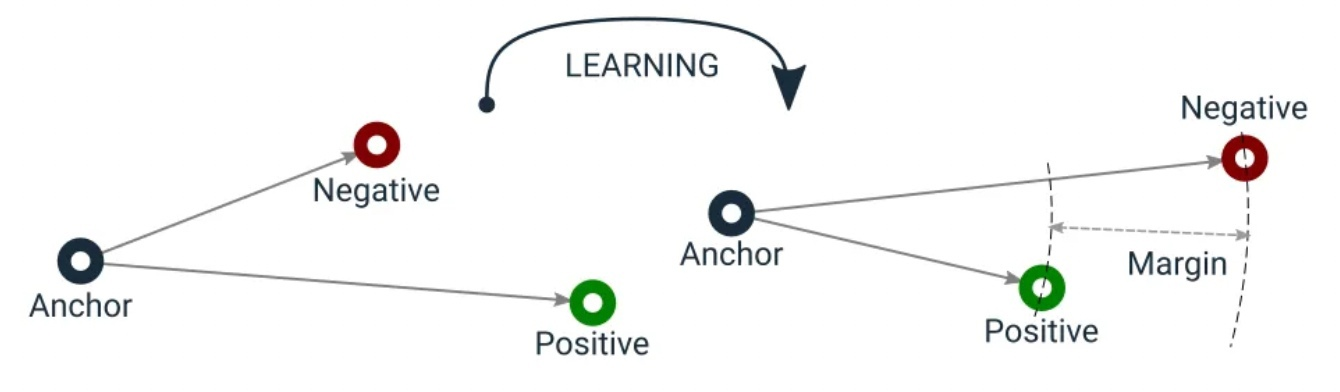
\includegraphics[width=.4\linewidth]{Images/triplet.jpeg}
  % \caption{Triplet loss visualization}
  \label{fig:sub1}
\end{subfigure}%
\begin{subfigure}
  \centering
  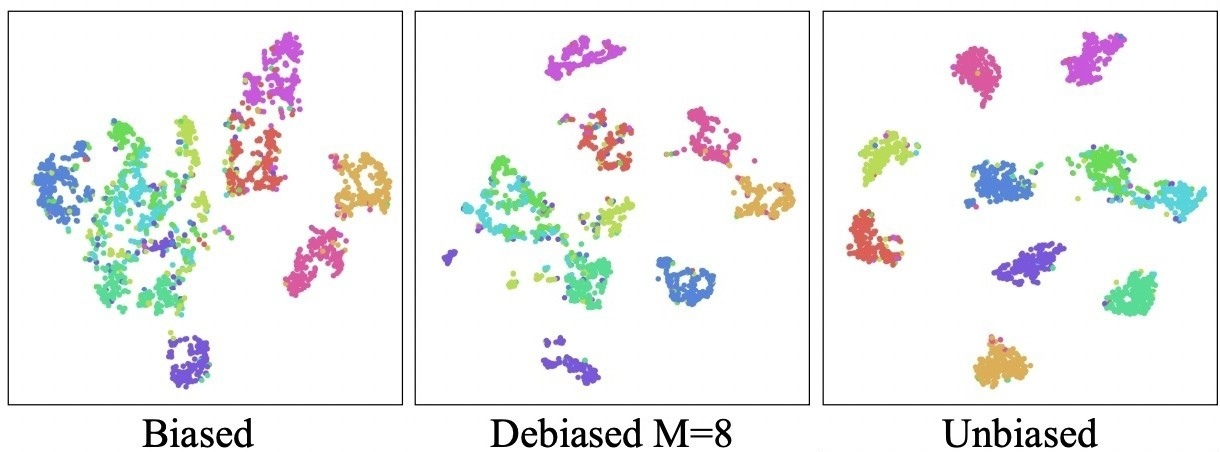
\includegraphics[width=.5\linewidth]{Images/t-SNE.jpeg}
  % \caption{t-SNE visualization of learned representations on CIFAR10}
  \label{fig:sub2}
\end{subfigure}
\label{fig:test}
\end{figure}

Найти $L_{\text{DebiasedPos}}^N$, минимизирующее $\lim \limits_{N \to \infty} \big|L_{\text{DebiasedPos}}^N (f)  - L_{\text{Unbiased}}^N(f)\big|$.

\begin{equation*} \small
L_{\text{Unbiased}}^N(f) = \mathbb{E}_{\substack{\mathbf{x} \sim p, \mathbf{x^+} \sim p^+_x,\\ \mathbf{x^-} \sim p_x^-}} \bigg[-\log \frac{\exp (\scriptsize\text{sim}_f(\mathbf{x}, \mathbf{x^+}))}{\exp (\scriptsize\text{sim}_f(\mathbf{x}, \mathbf{x^+}) + \sum _{i=1}^N \exp (\scriptsize\text{sim}_f(\mathbf{x}, \mathbf{x^-})}\bigg]
\end{equation*}

\end{frame}
%------------------------------------------------

\begin{frame} 
	\frametitle{Список литературы}
	
	\begin{thebibliography}{99} 
		\footnotesize
		
		\bibitem[Chuang, 2020]{p1}
			Ching-Yao Chuang, Joshua Robinson, Lin Yen-Chen, Antonio Torralba, Stefanie Jegelkah (2020)
			\newblock Debiased Contrastive Learning

            \bibitem[khosla2021supervised, 2020]{p2}
			Prannay Khosla, Piotr Teterwak, Chen Wang, Aaron Sarna, Yonglong Tian, Phillip Isola, Aaron Maschinot, Ce Liu, Dilip Krishnan (2021)
			\newblock Supervised Contrastive Learning

           \bibitem[Chen2020SimCLR, 2020]{p3}
			CTing Chen, Simon Kornblith, Mohammad Norouzi, Geoffrey Hinton (2020)
			\newblock A Simple Framework for Contrastive Learning of Visual Representations

   		\bibitem[Sohn, 2016]{p4}
			Sohn, Kihyuk (2016)
			\newblock Improved Deep Metric Learning with Multi-class N-pair Loss Objective

   		\bibitem[schroff2015facenet, 2015]{p5}
			Florian Schroff, Dmitry Kalenichenko, James Philbin (2015)
			\newblock FaceNet: A Unified Embedding for Face Recognition and Clustering

	\end{thebibliography}
\end{frame}
%------------------------------------------------

\begin{frame}
    \frametitle{Решение}
\scriptsize
Обозначим $h(\textbf{x}, \widetilde{\textbf{x}}) := e^{f(\textbf{x})^T f(\widetilde{\textbf{x}})}$.

\begin{lemma}
При $N \to \infty$:
\begin{equation*}
L_{\text{Unbiased}}^N(f) 
\longrightarrow
\mathbb{E}_{\substack{\textbf{x} \sim p \\ \textbf{x}^- \sim p_x^-}} \bigg[ - \log \frac{R}{R + N \color{blue} \mathbb{E}_{\textbf{x}^- \sim p_x^-} h(\textbf{x}, \textbf{x}^-)}\bigg],
\end{equation*}
где
\begin{equation*}
R = \frac{1}{\tau^+} \big(\color{violet} \mathbb{E}_{\textbf{x}' \sim p} h(\textbf{x}, \textbf{x}') \color{black}  - \tau^- \color{blue} \mathbb{E}_{\textbf{x}^- \sim p_x^-} h(\textbf{x}, \textbf{x}^-)\big).
\end{equation*}
\end{lemma}

\begin{equation*}
\tilde{L}_{\text{DebiasedPos}}^N (f) = \mathbb{E}_{\substack{\textbf{x} \sim p \\ \textbf{x}^- \sim p_x^-}} \bigg[ - \log \frac{\color{violet} \mathbb{E}_{\textbf{x}' \sim p} h(\textbf{x}, \textbf{x}') \color{black} - \tau^- \color{blue} \mathbb{E}_{\textbf{x}^- \sim p_x^-} h(\textbf{x}, \textbf{x}_i^-)}{\color{violet} \mathbb{E}_{\textbf{x}' \sim p} h(\textbf{x}, \textbf{x}') \color{black} + \big(N \tau^+ - \tau^-\big) \color{blue} \mathbb{E}_{\textbf{x}^- \sim p_x^-} h(\textbf{x}, \textbf{x}_i^-)}\bigg]
\end{equation*}

Оценим неизвестные матожидания эмпирически:
\begin{equation*}
\color{violet}P_{\text{emp}} (\textbf{x}, \{\textbf{u}_i\}_{i=1}^N, \textbf{v}) = \frac{1}{N+2} \bigg(\sum \limits_{i=1}^N h(\textbf{x}, \textbf{u}_i) + h(\textbf{x}, \textbf{v}) + h(\textbf{x}, \textbf{x})\bigg)\color{black}; \color{blue} P_{\text{emp}}^- (\textbf{x}, \{\textbf{u}_i\}_{i=1}^N) = \frac{1}{N} \sum \limits_{i=1}^N h(\textbf{x}, \textbf{u}_i).
\end{equation*}

\end{frame}
%------------------------------------------------

\begin{frame}
    \frametitle{Решение}
\scriptsize

\begin{equation*}
\tilde{L}_{\text{DebiasedPos}}^N (f) = \mathbb{E}_{\substack{\textbf{x} \sim p \\ \textbf{x}^- \sim p_x^-}} \bigg[ - \log \frac{\color{violet} \mathbb{E}_{\textbf{x}' \sim p} h(\textbf{x}, \textbf{x}') \color{black} - \tau^- \color{blue} \mathbb{E}_{\textbf{x}^- \sim p_x^-} h(\textbf{x}, \textbf{x}_i^-)}{\color{violet} \mathbb{E}_{\textbf{x}' \sim p} h(\textbf{x}, \textbf{x}') \color{black} + \big(N \tau^+ - \tau^-\big) \color{blue} \mathbb{E}_{\textbf{x}^- \sim p_x^-} h(\textbf{x}, \textbf{x}_i^-)}\bigg]
\end{equation*}

Финальная оценка:
\begin{equation*}
L_{\text{DebiasedPos}}^N (f) = \mathbb{E}_{\substack{\textbf{x} \sim p \\ \{\textbf{u}_i\}_{i=1}^N \sim {p_x^-}^N \\ \textbf{v} \sim p_x^+}} \bigg[-\log \frac{\color{violet}P_{\text{emp}} \color{black} - \tau^- \color{blue} P_{\text{emp}}^-} {\color{violet}P_{\text{emp}} \color{black} + \big(N \tau^+ - \tau^-\big) \color{blue} P_{\text{emp}}^- }\bigg].
\end{equation*}

\begin{theorem}
Для произвольного эмбеддинга f и произвольного $\delta > 0$ существует достаточно большое $N$, что
\begin{equation*}
\big|\tilde{L}_{\text{DebiasedPos}}^N (f) - L_{\text{DebiasedPos}}^N (f)\big| \leq \bigg[\bigg(1 + \frac{\tau^-}{\tau^+} + \delta\bigg) \sqrt{\frac{\pi}{2N}} + \bigg(1 + \frac{1}{\tau^+}\bigg) \sqrt{\frac{\pi}{2N + 2}}\bigg] e^{3/2}
\end{equation*}
\end{theorem}


\end{frame}
%------------------------------------------------

% \begin{frame}
% 	\frametitle{Debiased Contrastive Learning}
%  \framesubtitle{Ching-Yao Chuang et al., NeurIPS 2020} % Optional subtitle

% \scriptsize Минимизация $L_{\text{Debiased}}$ соответствует минимизации верхней границы $L_{\text{Unbiased}}$ в задаче обучения с учителем.

% \begin{equation*} \tiny
% L_{\text{Debiased}}^{N, M} (f) = \mathbb{E}_{\substack{\mathbf{x} \sim p; \mathbf{x}_+ \sim p_x^+,\\ \{\mathbf{u_i}\}_{i=1}^N \sim p^N \\ \{\mathbf{v_i}\}_{i=1}^M \sim p_x^+^M}}  \bigg[ -\log \frac{e^{f(\mathbf{x})^T f(\mathbf{x}^+)}}{e^{f(\mathbf{x})^T f(\mathbf{x}^+)} + N g\big(\mathbf{x}, \{\mathbf{u_i}\}_{i=1}^N, \{\mathbf{v_i}\}_{i=1}^M\big)} \bigg],
% \end{equation*}

% \begin{equation*} \tiny 
% g\bigg(\mathbf{x}, \{\mathbf{u_i}\}_{i=1}^N, \{\mathbf{v_i}\}_{i=1}^M\bigg) = \max \bigg\{ \frac{1}{\tau^-}\bigg(\frac{1}{N} \sum \limits_{i=1}^N e^{f(\mathbf{x})^T f(\mathbf{u_i})} - \tau^+ \frac{1}{M} \sum \limits_{i=1}^M e^{f(\mathbf{x})^T f(\mathbf{v_i})}\bigg), e^{-1/t}\bigg\}
% \end{equation*}

% \begin{figure}
%     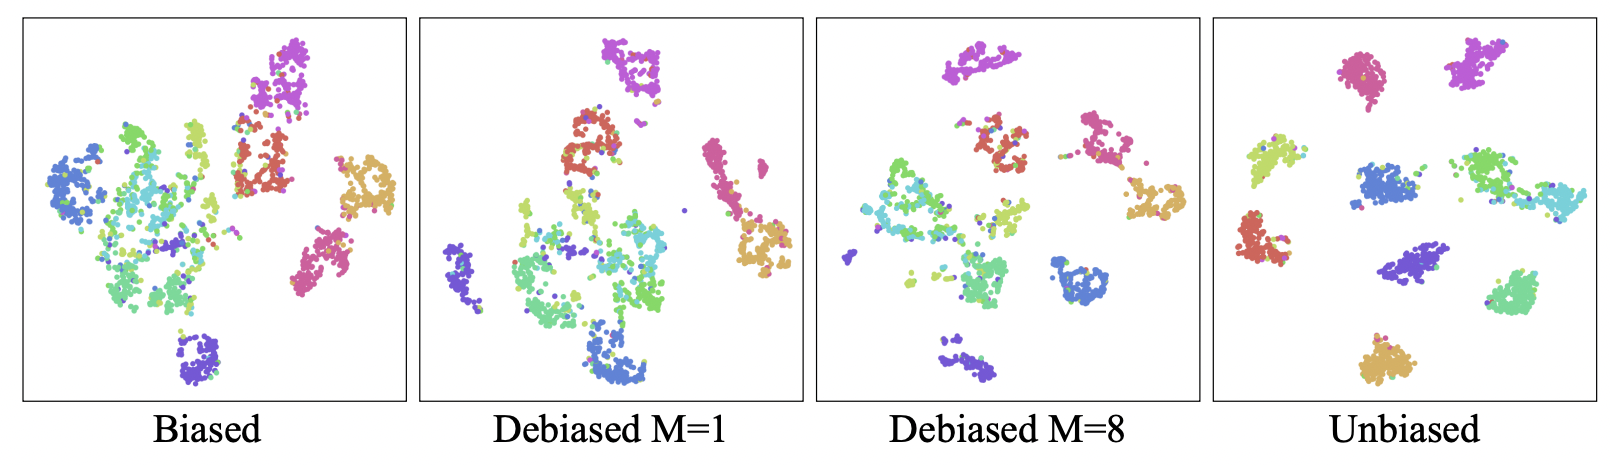
\includegraphics[width=0.7\linewidth]{Images/tsne.png}
% \end{figure}

% \end{frame}

%------------------------------------------------

\begin{frame}
	\frametitle{Использование SimCLR}
	\framesubtitle{CTing Chenet al., 2020} % Optional subtitle

\begin{figure}
    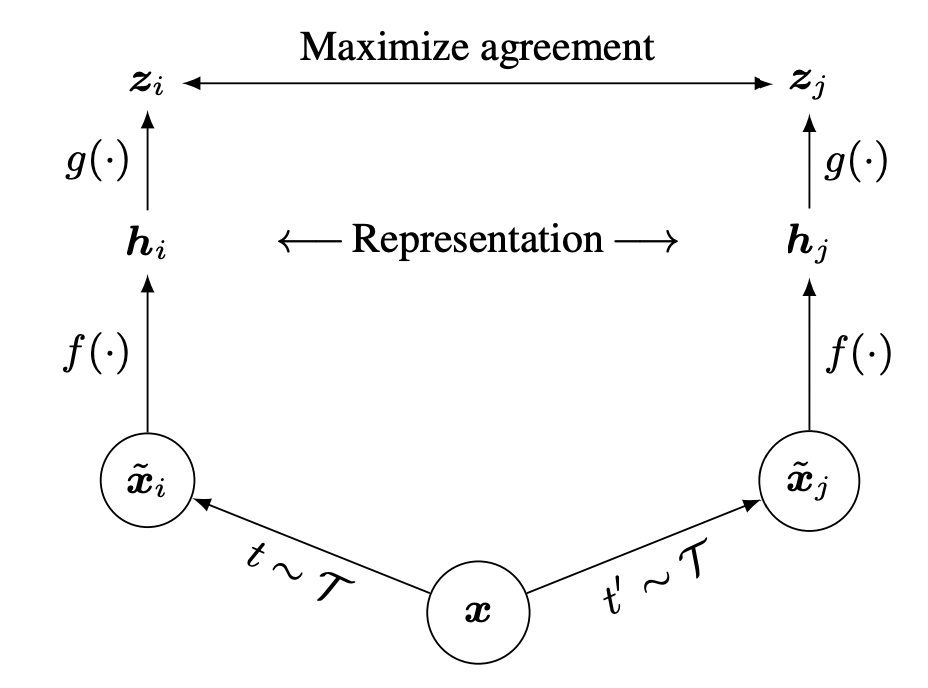
\includegraphics[width=0.5\linewidth]{Images/simclr.png}
\end{figure}

\scriptsize
\begin{itemize}
    \item $\mathcal{T} -$ семейство аугментаций (color distortion, gaussian blur) 
    \item Семплируются 2 аугментации $t, t' \sim \mathcal{T}$, применяются к каждому объекту.
    \item Обучаем сеть-энкодер $f(\cdot)$ и MLP сеть-проекцию $g(\cdot)$, максимизируя соответсвтие представлений.
\end{itemize}
\end{frame}

%------------------------------------------------

\begin{frame}
	\frametitle{Эксперимент с удалением FN и с добавлением FP}
\begin{figure}
\centering
\begin{subfigure}
  \centering
  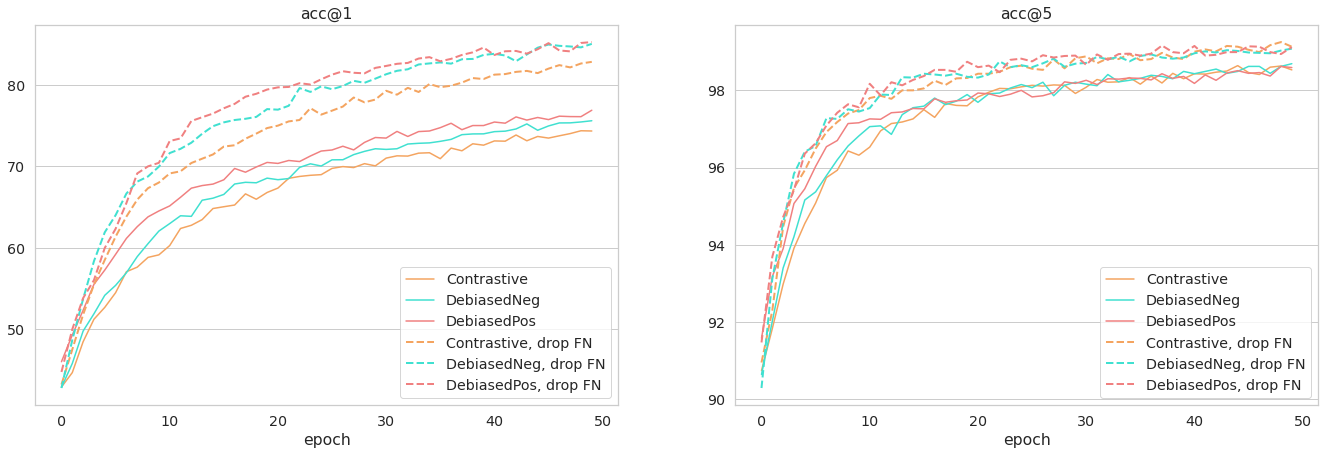
\includegraphics[width=0.95\linewidth]{Images/base_vs_dropfn.png}
  \label{fig:sub1}
\end{subfigure}%
\begin{subfigure}
  \centering
  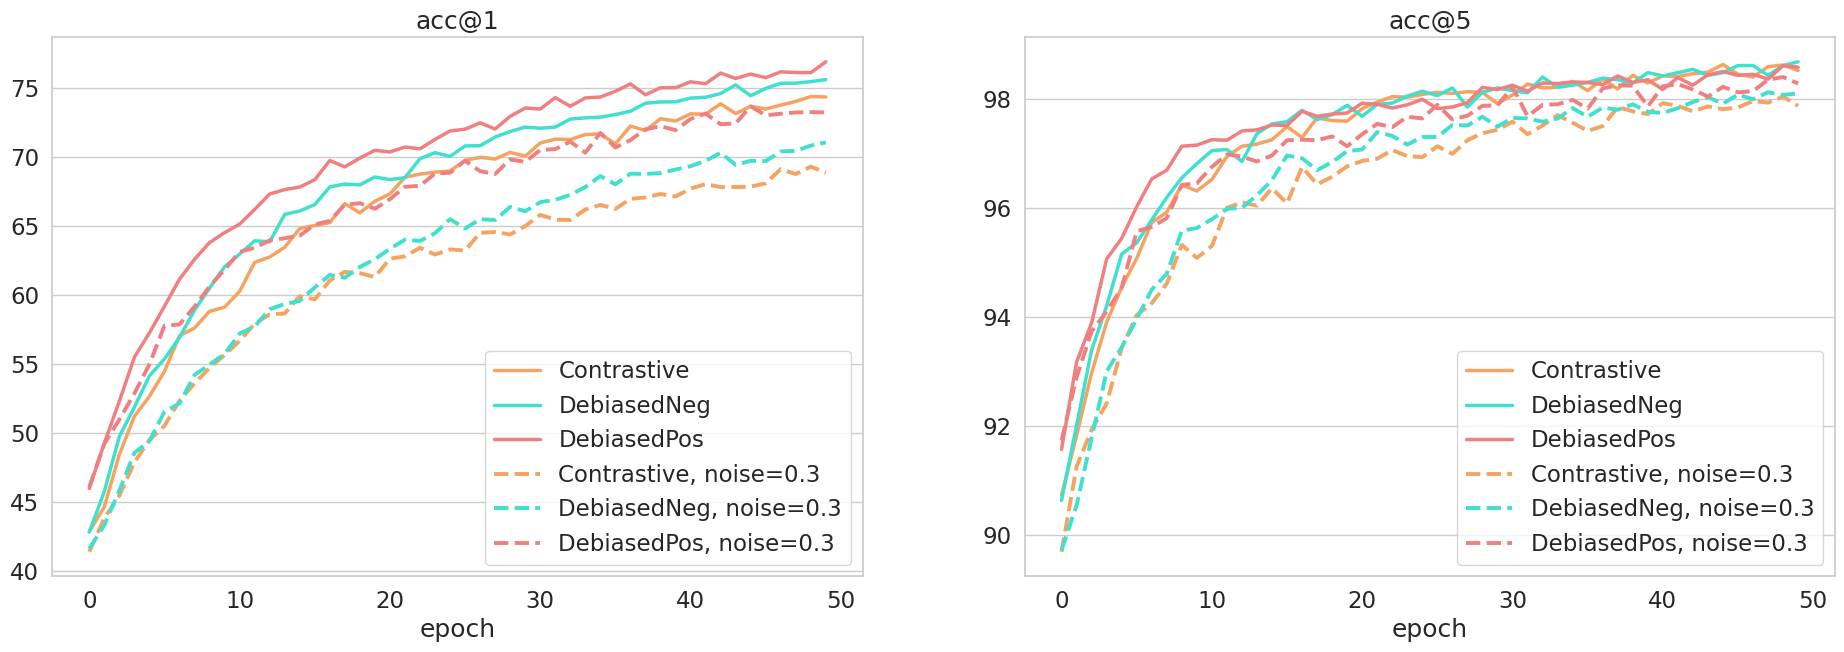
\includegraphics[width=0.95\linewidth]{Images/base_vs_noise.png}
  \label{fig:sub2}
\end{subfigure}
\label{fig:test}
\end{figure}
	
\end{frame}
%------------------------------------------------

\begin{frame}
	\frametitle{Эксперимент с увеличением кол-ва положительных семплов}
\begin{figure}
\centering
\begin{subfigure}
  \centering
  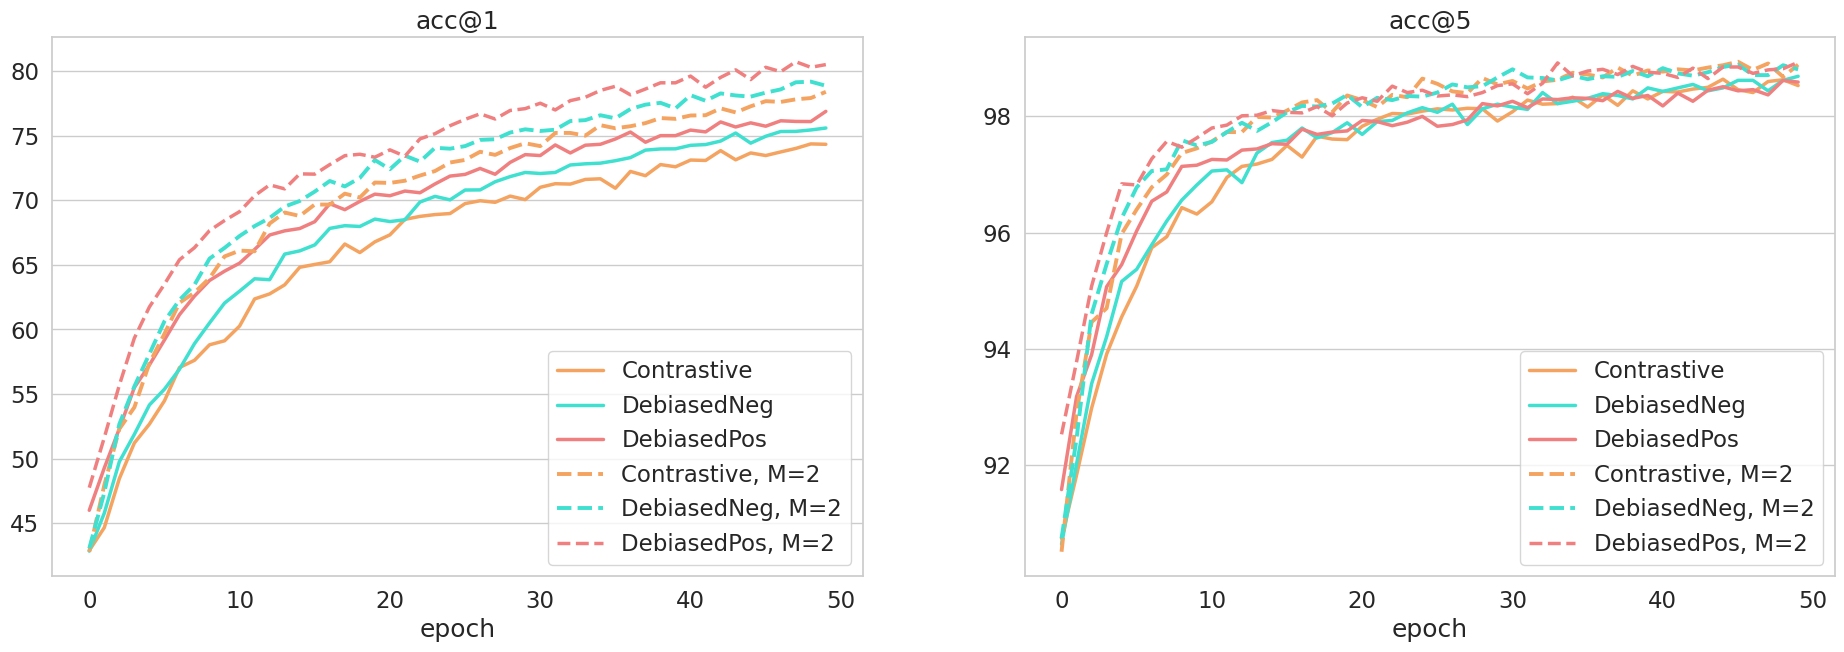
\includegraphics[width=1\linewidth]{Images/base_vs_M=2.png}
  \label{fig:sub1}
\end{subfigure}
\label{fig:test}
\end{figure}
	
\end{frame}
%------------------------------------------------

\begin{frame}
	\frametitle{Заключение}

\scriptisize

\begin{itemize}
    \item Лосс с устраненным FP-смещением добивается точности, сопоставимой с DebiasedNeg, и имеет превосходство на ранних эпохах.
    \item В случае удаления ошибок FN функции потерь DebiasedPos и DebiasedNeg имеют сопоставимые точности.
    \item При сильном зашумлении датасета, когда FP-rate увеличен, DebiasedPos имеет большое преимущество в точности над DebiasedNeg.
    \item При увеличенном кол-ве положитлеьных семплов точность для всех рассмотренных функций потерь возрастает.
\end{itemize}

\end{frame}

%------------------------------------------------------------------------------
%	CLOSING SLIDE
%------------------------------------------------------------------------------

% \begin{frame}[plain] % The optional argument 'plain' hides the headline and footline
% 	\begin{center}	
% 		\bigskip\bigskip % Vertical whitespace
% 		{\LARGE Спасибо за внимание!}
% 	\end{center}
% \end{frame}

%----------------------------------------------------------------------------------------

\end{document} 